%========================= CAPITULO 4 ==============================

\chapter{Aplicação} %\label{cap_exemplos}
%\thispagestyle{empty}
\section{Instalação do Asterisk}
A instalação do Asterisk requer e exige uma série de cuidados e detalhes,  para que se tenha um ambiente de telefonia estável e disponível o maior tempo possível. Logo, e necessário uma instalação onde busca-se a menor quantidade de problemas e com maior tempo operando, pois a compilação do Asterisk não é um processo trivial \cite{alexandrekeller2014}.

Apesar de haver duas formas de instalação, onde pode ser por SVN\footnote{Sistema de controle de versão} que mantêm um compartilhamento do desenvolvimento do sistemas com todas as novas funcionalidades, porém ainda nem sempre devidamente testadas, logo optou-se por baixar os pacotes compactados sendo eles:

\begin{itemize}
  \item dahdi-linux-current.tar.gz
  \item dahdi-tools-current.tar.gz
  \item libpri-1.4-current.tar.gz
  \item openr2-1.3.3.tar.gz
  \item libss7-1.0.2.tar.gz
  \item asterisk-13-current.tar.gz
\end{itemize}

E podem ser obtidos respectivamente nos seguintes endereços:

\begin{itemize}
  \item http://downloads.asterisk.org/pub/telephony/dahdi-linux/
  \item http://downloads.asterisk.org/pub/telephony/dahdi-tools/
  \item http://downloads.asterisk.org/pub/telephony/libpri/
  \item https://code.google.com/p/openr2/downloads/list
  \item http://downloads.asterisk.org/pub/telephony/libss7/
  \item http://downloads.asterisk.org/pub/telephony/asterisk/
\end{itemize}

Após o download dos mesmo foram descompactados e compilados na mesma ordem em que foram baixados, pois, os modulos são independentes, ou seja, a compilação de um módulo reflete diretamente na compilação do outro, a exemplo, caso seja compilado o módulo do Asterisk antes do módulo LIBPRI, a compilação do Asterisk não reconhecerá as funções habilitadas pelo pacote LIBPRI.

Após a instalação do Asterisk algumas pastas e arquivos são criados por ele para sua respectiva configuração e armazenamento das informações, pois o Asterisk é dividido em módulos, cada um representando uma funcionalidade como aplicação, função, canal de comunicação, protocolo e outros, e para correta configuração destas funcionalidades e necessário correta construção e configuração destes arquivos, e no decorrer do projeto, serão abordados os arquivos de configuração pertinentes para a correta construção do protótipo para ser testado no teleatendimento.

\subsection{Protótipo}
O protótipo consiste na construção de servidor PABX híbrido para o teleatendimento da Polícia Miltar de Dourados, onde serão configuradas as funcionalidades do Asterisk pertinentes a este teleatendimento, logo, serão apresentados os arquivos com as configurações necessárias para esta finalidade.

\subsubsection{Plano de Discagem}
O plano de discagem define todo o funcionamento do servidor Asterisk, é onde define os grupos e regras de discagem, ou seja, como as chamadas de entradas e saída do servidor serão tratadas, e quais funcionalidades serão atividades e como funcionarão, o arquivo onde é programado o plano de discagem é o ``extensions.conf'' e fica localizado dentro da pasta ``/etc/asterisk/'' \cite{alexandrekeller2014}.

Para o teleatendimento foi configurado uma URA com uma mensagem de boas vindas, ou seja, informando de qual órgão de segurança pública corresponde, neste caso a mensagem é “polícia militar”, e o originador da chamada cairá na fila de atendimento,  caso os todos atendentes estejam ocupados, informará através de uma mensagem que todos os atendentes estão ocupados e posteriormente a posição que originador da chamada se encontra dentro da fila. Caso um atendente esteja disponível a chamada ira ser direcionada para este atendente, e caso exista mais de um será escolhido o atendente que esta mais tempo sem atender uma chamada. A figura \ref{Figura19} ilustra a configuração do arquivo extension.conf referente a URA, onde foi criado um contexto chamado “uraprincipal” e neste contexto uma extensão que de forma sucessiva atendente a chamada, toca o arquivo de boasvindas e transfere a ligação para a fila de atendimento.

\begin{figure}[h]
	\centering
	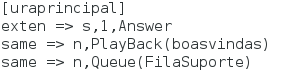
\includegraphics[width=8cm]{imagens/ura.png}
	\caption{Arquivo extension.conf configuração da URA.}
    \label{Figura19}
\end{figure}

No plano de discagem ou seja na configuração do arquivo extensions.conf ainda será necessário mais algumas modificações para o correto funcionamento do servidor Asterisk no teleatendimento, logo, as demais modificações serão abordadas juntos com os arquivos de outras funcionalidades como o arquivo ``dahdi-channels.conf''  responsável pela definição dos canais de comunicação da placa TDM410P para os Asterisk.

\subsubsection{Distribuição Automática das Chamadas (DAC)}
A DAC é a maneira pela qual o Asterisk proporciona o enfileiramento das chamadas de entrada no servidor, para que sejam encaminhadas para os atendentes \cite{books/daglib/0018909}.

Para a DAC do teleatendimento foi configura uma fila de atendimento que usa uma estratégia de atendimento onde o atendente que esta mais tempo sem atender uma chamada recebera a primeira chamada da fila assim de forma sucessiva. A figura \ref{Figura20} ilustra o arquivo ``queues.conf'' que está localizado dentro da pasta /etc/asterisk/.

\begin{figure}[h]
	\centering
	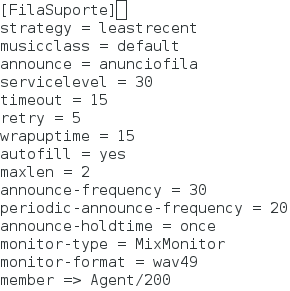
\includegraphics[width=7cm]{imagens/dac.png}
	\caption{Arquivo queues.conf configuração da DAC.}
    \label{Figura20}
\end{figure}

Dentre todas as configurações do arquivo queues.conf, se destaca o nome da fila, que é declarado como uma extensão de nome “[FilaSuporte]”, depois tem “strategy” que é definida como leastrecent, ou seja a estratégia de atendimento, e ainda ``monitor-format = wav49'', ou seja, define como wav49 a extensão do arquivo que será gravado o audio, e por fim ``member => Agent/200'', define os agente que compõe a fila, ou seja, os atendentes que poderão autenticar-se no servidor para atender uma chamada.

Para configurar os agentes faz necessário configurar também o arquivo ``agents.conf'' localizado na pasta ``/etc/asterisk/'', bem como configurar os ramais no arquivo extensions.conf, a figura \ref{Figura21} ilustra a configuração dos agentes para o teleatendimento, apesar de figura monstrar apenas um atendente, foi configurado o número exato de atendentes do teleatendimento, a figura \ref{Figura22} ilustra a configuração dos atendentes no arquivo extensions.conf.

\begin{figure}[h]
	\centering
	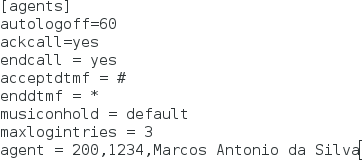
\includegraphics[width=7cm]{imagens/agents.png}
	\caption{Arquivo agents.conf configuração dos agentes de atendimento}
    \label{Figura21}
\end{figure}

\begin{figure}[h]
	\centering
	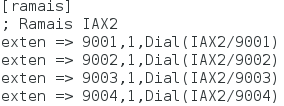
\includegraphics[width=6cm]{imagens/ramais.png}
	\caption{Arquivo extensions.conf configuração dos agentes de atendimento}
    \label{Figura22}
\end{figure}

É necessário ainda configurar o arquivo iax.conf, onde define o tipo de protocolo de comunicação, que para o teleatendimento foi escolhido o iax2, define-se também  neste arquivo os ramais que compõe o teleatendimento e os codecs de áudio, logo, foi utilizado o alaw e ildc. A figura \ref{Figura23} ilustra a configuração dos ramais no arquivo iax.conf.

\begin{figure}[h]
	\centering
	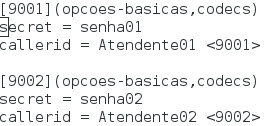
\includegraphics[width=6cm]{imagens/iax.png}
	\caption{Arquivo iax.conf configuração dos ramais}
    \label{Figura23}
\end{figure}

\subsubsection{Captura e Transferência de Chamadas}
Capturar uma chamada, significa transferir a chamada que está tocando em outro ramal, ou seja, de outro atendente, para o seu ramal e assim atendê-la \cite{alexandrekeller2014}.

Foi criado uma grupo para os atendentes logo pode-se capturar as chamadas tanto em grupo como direta. Para tanto é necessário configurar o arquivo ``features.conf'', este arquivo ainda serve para configurar outros serviços como correio de voz, música de espera, estacionamento de chamadas, transferência de chamadas, salas de conferencia e gravação de chamadas individuais, ou seja, quando não há uma fila de atendimento, configura-se a gravação das chamadas neste arquivo. A figura \ref{Figura24} ilustra a configuração da captura de chamada.

\begin{figure}[h]
	\centering
	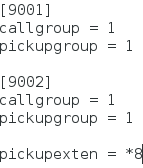
\includegraphics[width=3cm]{imagens/features.png}
	\caption{Arquivo features.conf configuração da captura de chamada}
    \label{Figura24}
\end{figure}

Há duas formas de transferência de chamadas, sendo as cegas onde não há a consulta prévia do destinatário da transferência ou assistida na qual é realizada uma consulta prévia do destinatário da transferência \cite{alexandrekeller2014}.

Optou-se em deixar as duas formas de transferência para o teleatendimento, a opção blindxfer = \#, define a transferência as cegas utilizando a tecla de sustenido, e a opção atxfer = *2 define a transferência assistida utilizando a junção das teclas asterisco mais o numeral 2 a figura \ref{Figura25} ilustra as opções que devem estar habilitadas no arquivo ``features.conf''.

\begin{figure}[h]
	\centering
	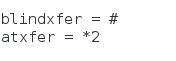
\includegraphics[width=4cm]{imagens/features2.png}
	\caption{Arquivo features.conf configuração da transferência de chamada}
    \label{Figura25}
\end{figure}

\subsubsection{Placa de Comunicação}
Para a placa comunicar com o Asterisk é necessário a configuração dos arquivos ``dahdi-channels.conf'' localizado em ``/etc/asterisk/'', onde este define os canais de comunicação, e o arquivo ``system.conf'' localizado em ``/etc/dahdi/'', onde este especifica como cada canal de comunicação ira se comunicar com o Kernel\footnote{O núcleo do Linux, forma a estrutura base do sistema operacional}.

As figuras \ref{Figura26} e \ref{Figura27} ilustram como ficou a configuração dos arquivos ``dahdi-channels.conf'' e ``system.conf'' respectivamente para atender o projeto do teleatendimento.

\begin{figure}[h]
	\centering
	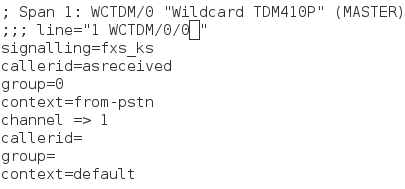
\includegraphics[width=8.5cm]{imagens/dahdi-chan.png}
	\caption{Arquivo dahdi-channels.conf configuração dos canais de comunicação}
    \label{Figura26}
\end{figure}

\begin{figure}[h]
	\centering
	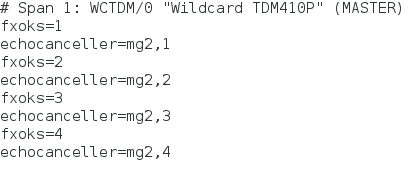
\includegraphics[width=8.5cm]{imagens/system.png}
	\caption{Arquivo system.conf configuração de cada canal com o Kernel}
    \label{Figura27}
\end{figure}

\subsubsection{Bilhetagem}
A bilhetagem é uma das principais funcionalidades do Asterisk pois permite armazenar todas as informações das chamadas de entrada e saída do servidor, podem ser uma simples arquivo de texto, como ser integrado a uma banco de dados externo \cite{flavioeduardoandredade2005}.

Para o teste realizado no teleatendimento, permaneceu o armazenamento em um arquivo de texto simples, porém para posterior emprego do servidor Asterisk neste teleatendimento pretende-se migar para o armazenamento externo através do banco de dados MySQL via conexão ODBC. Foi necessário a configuração do arquivo ``cdr.conf'', localizado na pasta ``/etc/asterisk'', os arquivos gerados ficam armazenados na pasta ``/vas/log/asterisk/crd-csv/''. A figura \ref{Figura28} ilustra a configuração do arquivo ``cdr.conf''.

\begin{figure}[h]
	\centering
	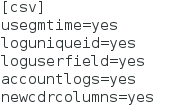
\includegraphics[width=4cm]{imagens/cdr.png}
	\caption{Arquivo cdr.conf configuração da bilhetagem}
    \label{Figura28}
\end{figure}

A figura 29 ilustra o arquivo master.csv, com a entrada de uma chamada, e exemplificando os paramentos mais pertinentes temos o \textit{calldat}, é a data da chamada, \textit{src}, é o número do originador da chamada, \textit{dst}, é quem recebeu a chamada, \textit{duration}, é o tempo que o originador permaneceu deste que caiu na fila até o fim do atendimento, \textit{billsec}, é o tempo que originador foi atendido pelo atendente, \textit{uniqueid}, é o identificador da chamada, ou seja é uma número único que é gerado para cada chamada.

\begin{figure}[h]
	\centering
	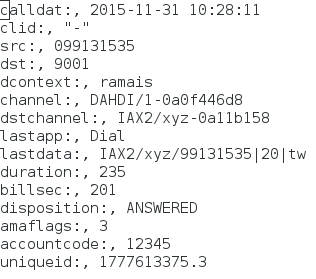
\includegraphics[width=7cm]{imagens/master.png}
	\caption{Arquivo master.csv entrada de uma chamada}
    \label{Figura29}
\end{figure}

\subsubsection{Estações de Trabalho dos Atendentes}
As estações de trabalhos dos atendentes já estão aptas para o emprego do teste no teleatendimento, a única configuração necessária foi ter que instalar o softfone nas estações e aquisição de headsets para o recebimento das chamadas.

O softfone escolhido foi o zoiper, pois o mesmo tem a possibilidade de configuração para os protocolos SIP e IAX2, e para o teste realizado no teleatendimento foi utilizado o procolo IAX2. A figura \ref{Figura30} ilustra o softfone apto a receber chamadas.

\begin{figure}[h]
	\centering
	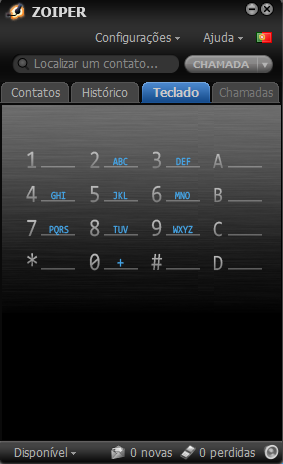
\includegraphics[width=4cm]{imagens/zoiper.png}
	\caption{Softfone instalado nas estações de trabalho}
    \label{Figura30}
\end{figure}

\subsubsection{Resultados Obtidos}
O servidor Asterisk foi aplicado por curto período de teste no teleatendimento, pois se trata de um protótipo, mas observou que o mesmo pode cumprir com a finalidade pretendida, que foi suprir as falhas observadas neste teleatendimento, através das funcionalidades que o mesmo possui e as quais foram configuradas pertinentes a necessidade deste teleatendimento.

A qualidade do áudio foi também surpreendente, bem como o número de informações armazenadas pela bilhetagem, a fila também se mostrou promissora pois o cidadão pode já de inicio identificar qual órgão de segurança pública desde o início da chamada, e ainda tem uma posição de onde esta na fila.
